
% POSTER EXAMPLE
%
% This is an example of a relatively sane poster. The box structure (and the
% narrative in general) is what I would expect, but it is completely
% non-mandatory; you may include whatever you want. Preferably, erase the
% existing box structure after you read it, and start from scratch.
%
% The main communication requirements for the poster that should be satisfied
% are as such:
%
% - At the defense, it should help you talk for around 10 minutes about your
%   thesis, and convince the committee that you did something interesting and
%   sufficiently complicated. Prepare pictures that explain your main results.
%
% - It should quickly communicate the main idea of your thesis to a random
%   educated by-walker. Ideally, a moderately-witted MFF graduate who has never
%   heard about your thesis before should be able to get the main "rough idea"
%   in less than 1 minute by just looking at the poster.

% modify the fontscale parameter to make everything slighly bigger or smaller.
\documentclass[portrait,a0paper,fontscale=0.25]{baposter}

\usepackage[utf8]{inputenc}
\usepackage[T1]{fontenc}

% FONT CHOICES
% Posters do not need to be PDF/A; you can choose any relatable font from the
% TeX font catalogue without much risk. Sans-serif fonts are suggested for the
% posters; see https://tug.org/FontCatalogue/sansseriffonts.html
\usepackage[sfdefault]{Fira Sans}
%\usepackage[default]{droidsans}
%\usepackage[math]{iwona}
%\usepackage[defaultfam]{montserrat}
%\usepackage{cmbright}
%\usepackage{yfonts}\renewcommand{\familydefault}{\frakdefault}

\usepackage{color}
\usepackage{graphicx}
\usepackage{amssymb,amsmath}
\usepackage[export]{adjustbox} %allows using valign with \includegraphics
\usepackage{subfig}

\renewcommand{\arraystretch}{1.5}

\usetikzlibrary{positioning}

% A WORD ABOUT COLORS
%
% This template is prepared with a relatively neutral gray background that
% gives decent box borders (with white and darker gray), does not clash with
% many colors (except for violet-brown and other mushroomish colors, perhaps)
% and gives a lot of space for highlighting stuff.
%
% Generally, other color variations are good too; there are no strict rules on
% the colors. Good choices include:
%
% - white backgrounds and differentiation of box headers by color (see
%   headerFontColor)
%
% - various slightly tinted backgrounds (try red!10 instead of black!3)
% 
% - dark backgrounds
%
% Keep in mind:
% - The normal "informative" text and figures should be DARK on LIGHT
%   background, not the other way around.
%
% - If you want a dark background, soften (darken) the box backgrounds a bit so
%   that they do not "shine" too much from the poster. Use \color{white} for
%   the heading, and switch the UK/MFF logos to white (see contents of logos/).
%
% - Do not mix too many color hues together. Most hues have their widely
%   accepted meaning (green: good result, red: problem, blue: information,
%   yellow: highlighter, brown: serious problem, violet: something really
%   weird/interesting/magic, depending on the shade).

\begin{document}

\color{black!80} % default font color
\begin{poster}{grid=false,
	eyecatcher=true,
	background=plain,
	bgColorOne=black!3, % background color
	columns=2,
	headerborder=none,
	textborder=none,
	headershape=rectangle,
	headershade=plain,
	boxshade=plain,
	boxColorOne=white,
	headershade=plain,
	headerColorOne=black!15, % box header background color
	headerFontColor=black,
	}%
	{
\includegraphics[height=7em]{logos/mff-black.pdf}}
	{Configurable point rasterization for large scatterplots}
	{\vspace{1ex} Tereza Kulichová}
	{
\includegraphics[height=7em]{logos/uk-red.pdf}}


%
% LEFT COLUMN
%

\begin{posterbox}[column=0,name=background,
headerColorOne=red!60, boxColorOne=red!20]{Background}
Until recently, scatterplots could only be plotted in R using its very slow base plot function. 

The \textbf{speed} problem was solved by package \texttt{scattermore}. However, \texttt{scattermore} had only a single-purpose \textbf{API} and it didn't prevent \textbf{overplotting} -- overlapping of the data in the visualization, making it difficult to see individual data.

The problem of overplotting, its symmetric case, and its primitive insufficient solution by randomizing point order are visible below.

\begin{center}
\setcaptiontype{figure}% Fake a figure environment
{\frame{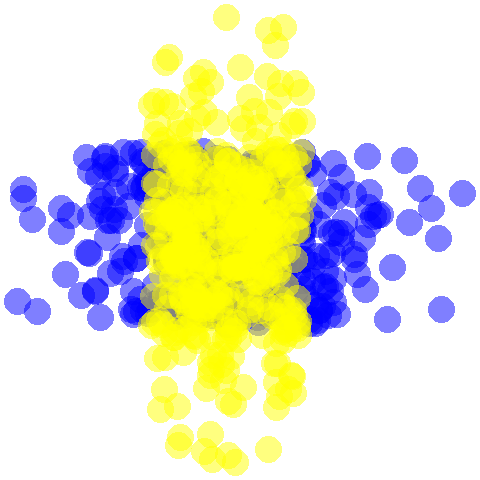
\includegraphics[width=0.25\linewidth]{img/overplot_yellow.png}}}
\hfill
{\frame{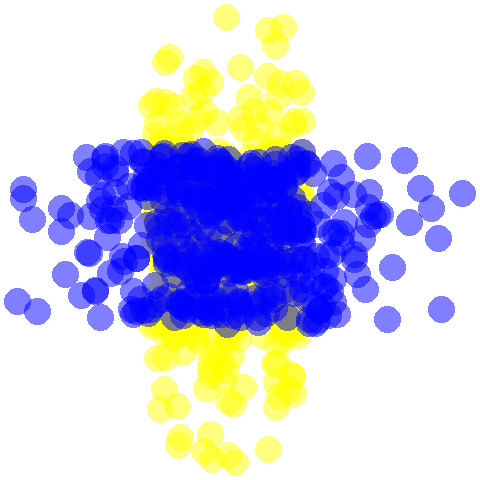
\includegraphics[width=0.25\linewidth]{img/overplot_blue.png}}}
\hfill
{\frame{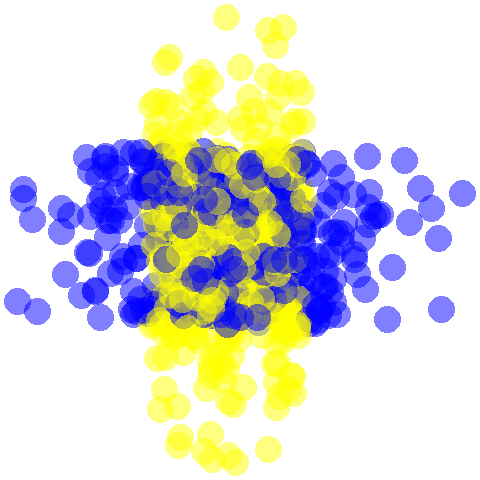
\includegraphics[width=0.25\linewidth]{img/overplot_random.png}}}
%\caption{Example of overplotting and techniques dealing with it.}
\end{center}

\end{posterbox}

\begin{posterbox}[column=0, name=goals, below=background, headerColorOne=cyan!60, boxColorOne=cyan!20]{Thesis goals}

We redesign \texttt{scattermore} with the following requirements.

\begin{itemize}
\item \textbf{High-customizable API.} We assign each subtask to a single method to ensure more variation in output for the user.
\item \textbf{Reduction of overplotting.} We introduce the new RGBWT data format, which combines images equally.
\item \textbf{Fast plotting.} We implement the computationally expensive operation in C language.
\end{itemize}

\end{posterbox}

\begin{posterbox}[column=0, name=pipeline, below=goals, 
headerColorOne=black!80, headerFontColor=white]{Scattermore pipeline}
\tikzstyle{box}=[rectangle,draw,rounded corners=0.5ex]
\tikzstyle{round}=[circle,draw, align=center]
\begin{center}\begin{tikzpicture}[thick,font=\sf\scriptsize]
\node[box,fill=pink!20] (input_no_colors_points) at (-2,12) {Points without color input};
\node[box,fill=pink!20] (input_no_colors_lines) at (-2,10) {Lines without color input};
\node[box,fill=black!10] (input_colors_points) at (-2,9) {Points with color input};
\node[box,fill=black!10] (input_colors_lines) at (-2,7) {Lines with color input};
\node[box,fill=red!30] (result) at (-2,5) {Raster result};
\node[round,fill=yellow!20] (histogram) at (2,12) {Histogram\\raster};
\node[round,fill=yellow!20] (blurred_histogram) at (5,12) {Kernelized\\histogram};
\node[round,fill=orange!20] (colorized_histogram) at (4,10) {RGBWT\\raster};
\node[round,fill=orange!20] (colorized_data) at (2,8) {RGBWT\\raster};
\node[round,fill=orange!20] (merged_rgbwt) at (5,8) {Merged\\RGBWT};
\node[round,fill=orange!20] (blurred_rgbwt) at (5,5) {Kernelized\\RGBWT};
\node[round,fill=purple!20] (rgba_int) at (1,5) {Integer\\RGBA};
\node[round,fill=green!20] (rgba_float) at (5,2) {Float\\RGBA};
\node[round,fill=green!20] (blended_rgba) at (0,2) {Blended\\float RGBA};

\draw[->](input_no_colors_points) to node[above=20pt, midway, sloped, font=\tiny\ttfamily] {scatter\_points\_histogram} (histogram);

\draw[->](input_no_colors_lines) to node[above=10pt, midway, sloped, font=\tiny\ttfamily] {scatter\_lines\_histogram} (histogram);

\draw[->](histogram) to node[above=20pt, midway, sloped, font=\tiny\ttfamily] {apply\_kernel\_histogram} (blurred_histogram);

\draw[->](blurred_histogram) to node[below=15pt, midway, sloped, font=\tiny\ttfamily] {histogram\_to\_rgbwt} (colorized_histogram);

\draw[->,dotted](histogram) to node[below=10pt, midway, sloped, font=\tiny\ttfamily] {histogram\_to\_rgbwt} (colorized_histogram);

\draw[->](input_colors_points) to node[above=15pt, midway, sloped, font=\tiny\ttfamily] {scatter\_points\_rgbwt} (colorized_data);

\draw[->](input_colors_lines) to node[above=10pt, midway, sloped, font=\tiny\ttfamily] {scatter\_lines\_rgbwt} (colorized_data);

\draw[->](colorized_data) to node[above=10pt, midway, sloped, font=\tiny\ttfamily] {merge\_rgbwt} (merged_rgbwt);

\draw[->](colorized_histogram) to node[above=10pt, midway, sloped, font=\tiny\ttfamily] {merge\_rgbwt} (merged_rgbwt);

\draw[->](merged_rgbwt) to node[above=10pt, midway, sloped, font=\tiny\ttfamily] {apply\_kernel\_rgbwt} (blurred_rgbwt);

\draw[->,dotted](blurred_rgbwt) to node[below=10pt, midway, sloped, font=\tiny\ttfamily] {rgbwt\_to\_rgba\_int} (rgba_int);

\draw[->](blurred_rgbwt) to node[above=10pt, midway, sloped, font=\tiny\ttfamily] {rgbwt\_to\_rgba\_float} (rgba_float);

\draw[->,dotted](colorized_histogram) to node[below=10pt, left, sloped, font=\tiny\ttfamily] {rgbwt\_to\_rgba\_int} (rgba_int);

\draw[->,dotted](colorized_data) to node[above=10pt, midway, sloped, font=\tiny\ttfamily] {rgbwt\_to\_rgba\_int} (rgba_int);

\draw[->,dotted](merged_rgbwt) to node[below=10pt, midway, sloped, font=\tiny\ttfamily] {rgbwt\_to\_rgba\_int} (rgba_int);

\draw[->,dotted](rgba_float) to node[below=10pt, midway, sloped, font=\tiny\ttfamily] {rgba\_float\_to\_rgba\_int} (rgba_int);

\draw[->](rgba_float) to node[below=10pt, midway, sloped, font=\tiny\ttfamily] {blend\_rgba\_float} (blended_rgba);

\draw[->](blended_rgba) to node[above=10pt, midway, sloped, font=\tiny\ttfamily] {rgba\_float\_to\_rgba\_int} (rgba_int);

\draw[->](rgba_int) to node[above=10pt, midway, sloped, font=\tiny\ttfamily] {rgba\_int\_to\_raster} (result);

\end{tikzpicture}\end{center}
\end{posterbox}


%
% RIGHT COLUMN
%
% It is usually best to fill most of the poster with your results and
% conclusions. Again, use simple annotated pictures wherever possible. Plots
% with measurements are perfect, tables are also good.
%

\begin{posterbox}[column=1, name=overplotting_api, headerColorOne=black!80, headerFontColor=white]{Result: Solution to overplotting and better API}
\begin{center}
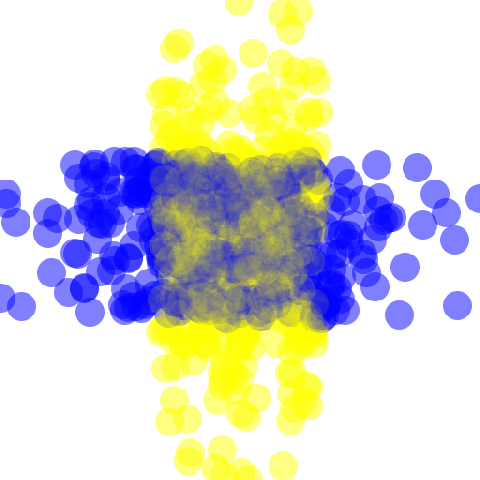
\includegraphics[width=0.3\linewidth]{img/overplot_merge.png}
\end{center}
\end{posterbox}


\begin{posterbox}[column=1, name=plot, below=overplotting_api, headerColorOne=black!80, headerFontColor=white]{Result: Improved Performance}
\begin{center}
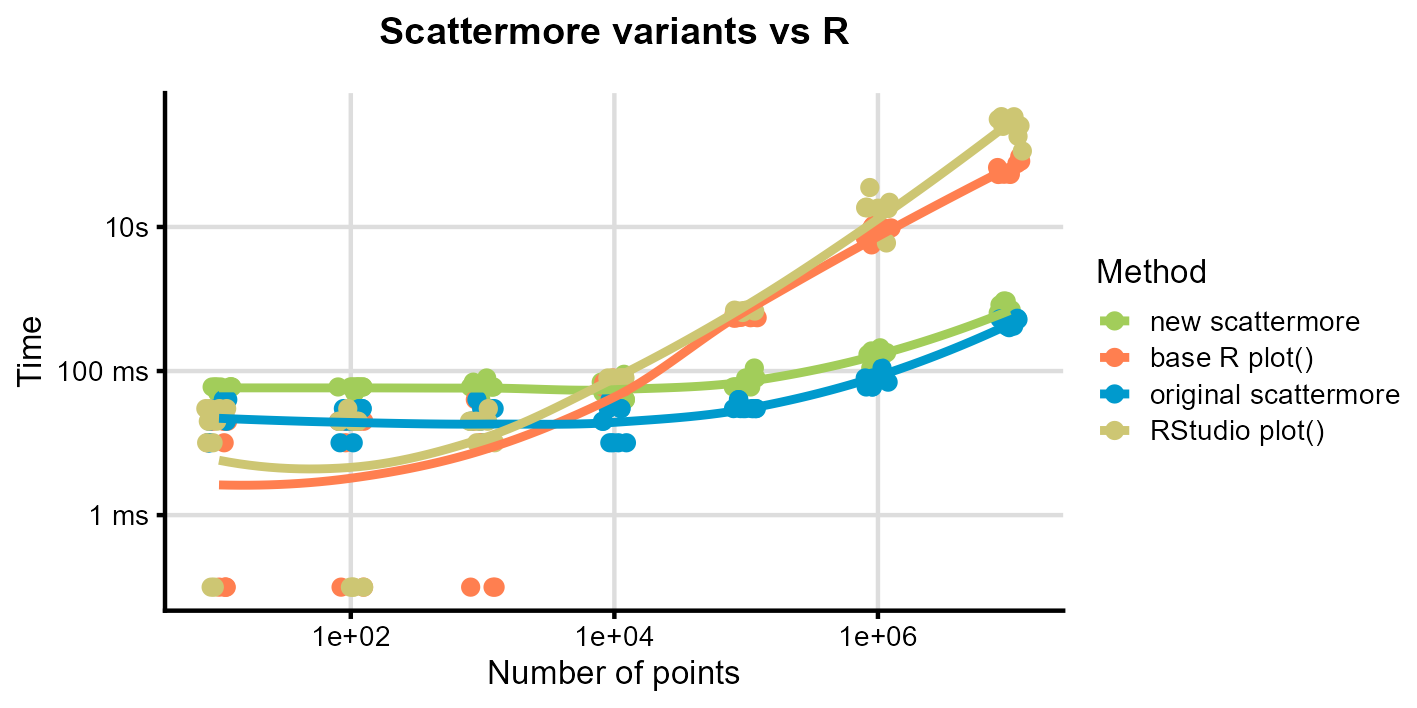
\includegraphics[width=0.7\linewidth]{img/version_comparison.png}
\end{center}

Comparison of the speed difference when plotting points among R, RStudio, original, and new \texttt{scattermore}’s version.
\end{posterbox}


\begin{posterbox}[column=1, name=main_result, below=plot, headerColorOne=green!90, boxColorOne=green!20]{Main result}
\large\bfseries
\vspace{1ex}
\begin{center}
% Program ThesisProgram solves the problem better than OtherProgram if X, and faster if Y.
Scattermore offers a highly customizable API, solves the problem of overplotting, and is much faster than base R functions.
\end{center}
\vspace{.5ex}
\end{posterbox}

\begin{posterbox}[column=1, name=conclusion, below=main_result, bottomaligned=pipeline, headerColorOne=violet!50, boxColorOne=violet!20]{Conclusions}
\begin{itemize}
\item \texttt{Scattermore} enables users to blur images, blend or merge them according to their preferences and, at the same time, sufficiently fast.
\item It is especially useful in the cytometric community for interactive analysis of large biological data.
\item \texttt{Scattermore} is available on GitHub as a development version and as R's official CRAN package version.
\end{itemize}
\textbf{Possible future work:}
\begin{itemize}
\item Working directly with 32-bit float data, avoiding the frequent conversions to 64-bit floats used in R.
\item Porting some operations to GPU.
\item Possibility to plot Bezier curves and filled polygons.
\end{itemize}
\begin{center}
\frame{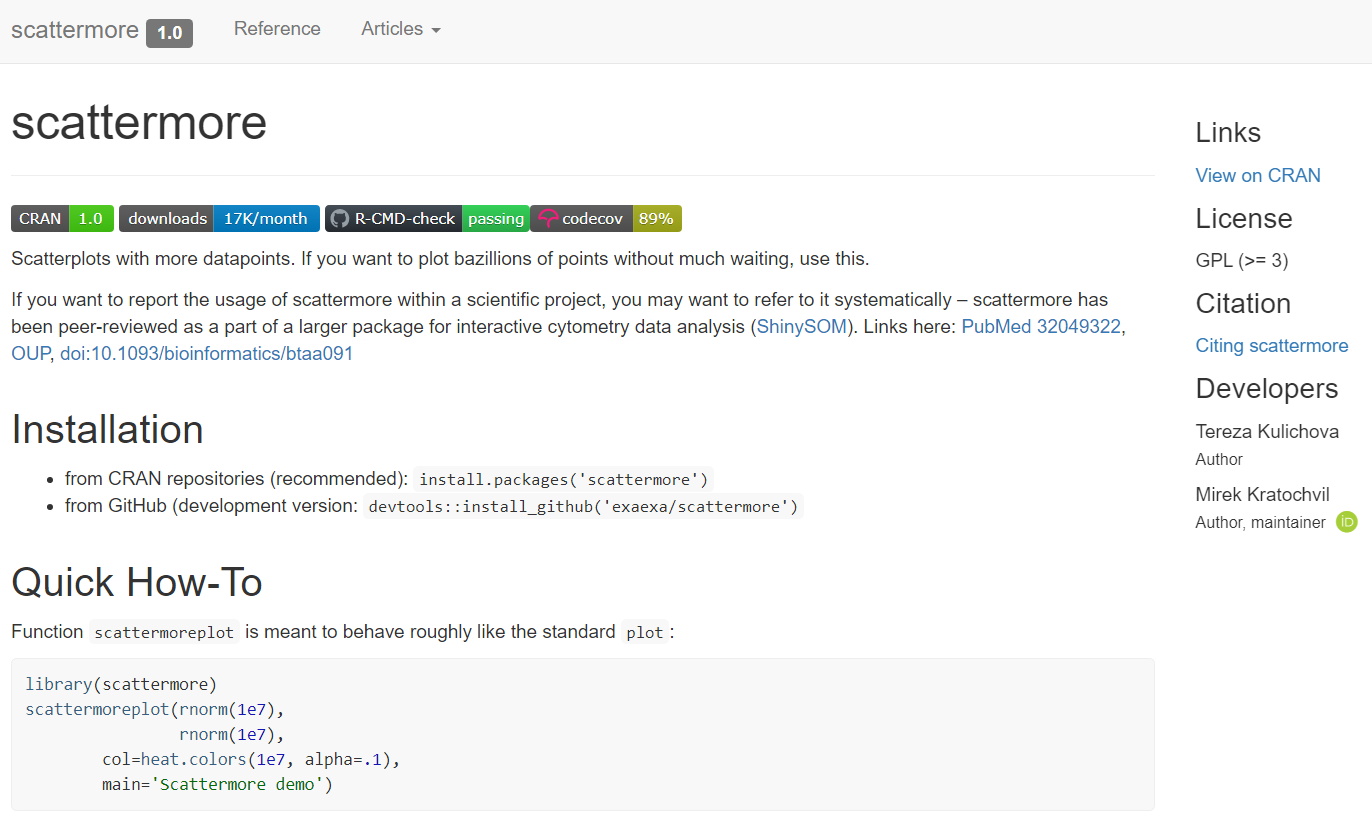
\includegraphics[width=0.55\linewidth]{img/github_scattermore.png}}
%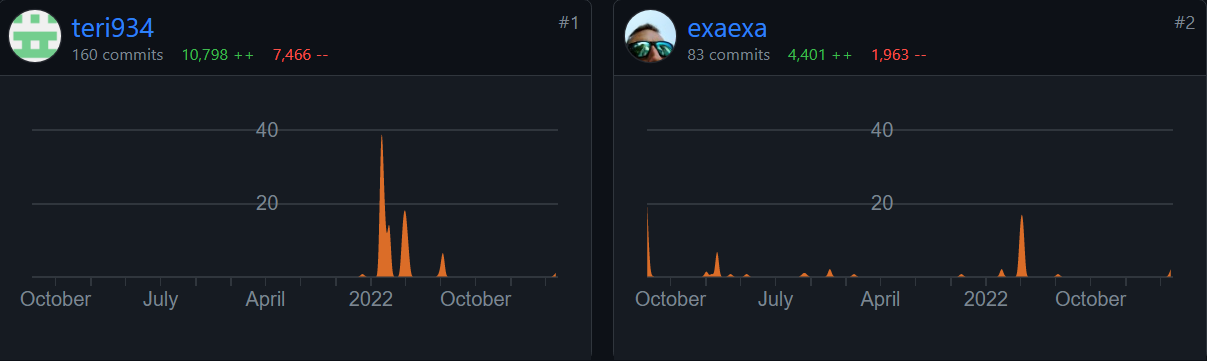
\includegraphics[width=0.5\linewidth]{img/github_contributions.png}
\end{center}
\end{posterbox}

\end{poster}
\end{document}
